\documentclass[Second Project.tex]{subfiles}

\begin{document}
\subsection{ Εκτίμηση της τιμής κλεισίματος της μετοχής της εταιρείας \textbf{ΕΛΛΗΝΙΚΑ ΠΕΤΡΕΛΑΙΑ} }
Στον πίνακα του \textit{Σχήματος 7} παρουσιάζονται οι τιμές κλείσιματος της μετοχής της 
\textbf{ΕΛΛΗΝΙΚΑ ΠΕΤΡΕΛΑΙΑ} για την περίοδο από τις 4 έως τις 24 Μαρτίου 2020.
\begin{figure}[h!]
    \centering
    \captionsetup{justification=centering}
    \begin{center}
        \begin{tabular}{ |c|c| } 
        \hline
        Ημερομηνία & Τιμή Κλείσιματος Μετοχής \\ \hline
        4 Μαρτίου 2020 & 6.81 \\ \hline
        5 Μαρτίου 2020 & 6.31 \\ \hline
        6 Μαρτίου 2020 & 6.02 \\  \hline
        9 Μαρτίου 2020 & 4.96 \\ \hline
        10 Μαρτίου 2020 & 5.35 \\  \hline
        11 Μαρτίου 2020 & 5.2 \\ \hline
        12 Μαρτίου 2020 & 4.82 \\ \hline
        13 Μαρτίου 2020 & 4.98 \\ \hline
        16 Μαρτίου 2020 & 4.65 \\ \hline
        17 Μαρτίου 2020 & 4.695 \\ \hline
        18 Μαρτίου 2020 & 4.555 \\ \hline
        19 Μαρτίου 2020 & 4.795 \\ \hline
        20 Μαρτίου 2020 & 5.35 \\ \hline
        23 Μαρτίου 2020 & 4.98 \\ \hline
        24 Μαρτίου 2020 & 5.28 \\ \hline
        \hline
        \end{tabular}
        \caption{Τιμές κλεισίματος της μετοχής της εταιρείας \textbf{ΕΛΛΗΝΙΚΑ ΠΕΤΡΕΛΑΙΑ}}
    \end{center}
\end{figure}

Στο αρχείο \textlatin{\textbf{hellenic\_petroleum\_stock.py}} χρησιμοποιώντας τις συναρτήσεις που αναπτύχθηκαν στην 
\textbf{Άσκηση 5} στην παράγραφο με την μέθοδο των ελαχίστων τετραγώνων και τις τιμές κλεισίματος από τις 4 έως 
και τις 17 Μάρτιου 2020 καταλήγουμε στα διαγράμματα των \textit{σχημάτων 8 και 9}.
\begin{figure}[h!]
    \centering
    \captionsetup{justification=centering}
    \subfloat{{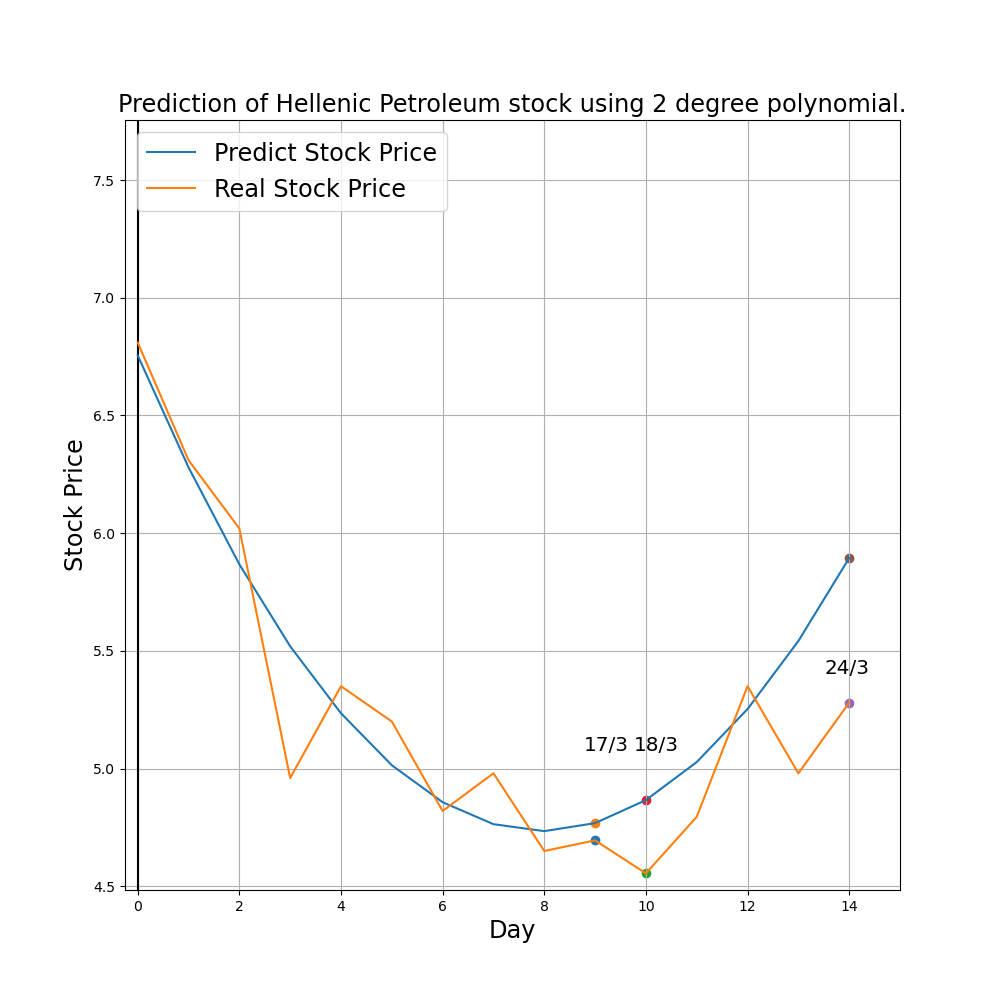
\includegraphics[scale=0.21]{hellenic_petroleum_stock_2_degree.png}}}
    \quad
    \subfloat{{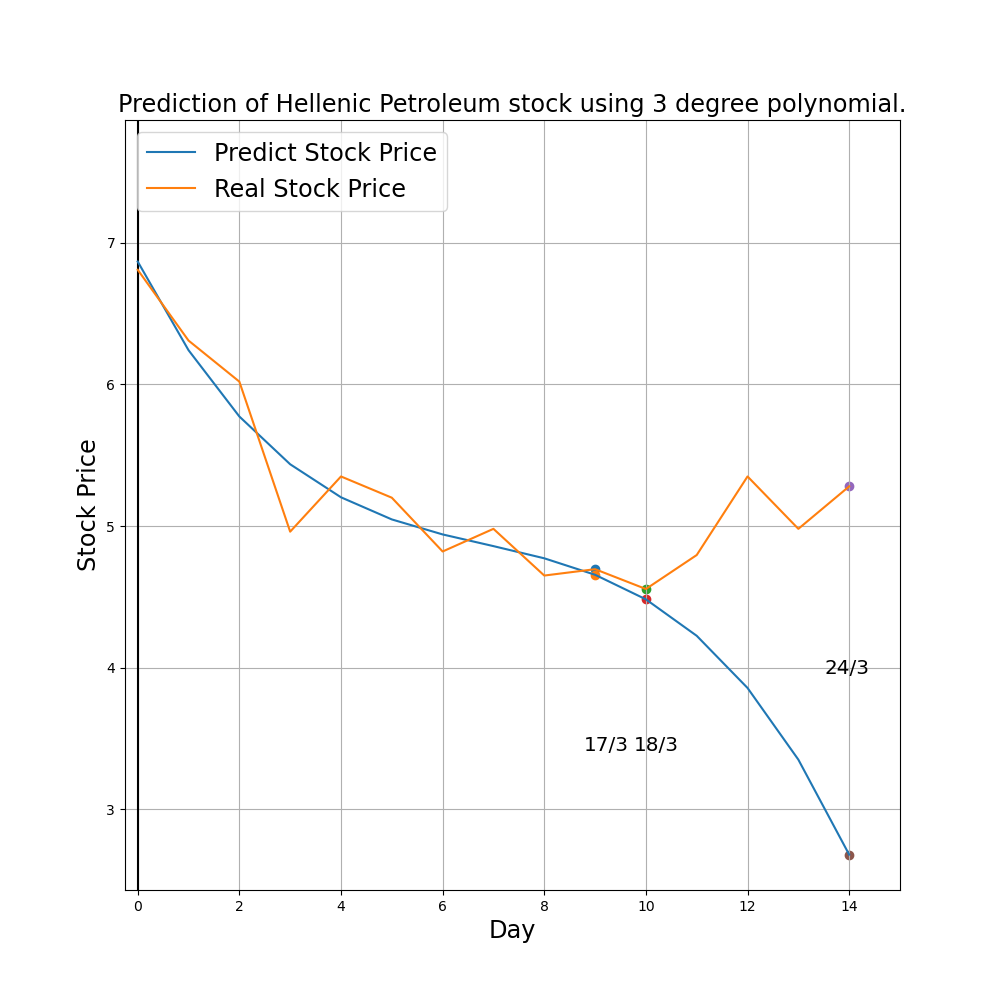
\includegraphics[scale=0.21]{hellenic_petroleum_stock_3_degree.png} }}
    \caption{ Διάγραμμα της πρόβλεψης καθώς και της πραγματικής τιμής κλεισίματος της μετόχης της εταιρείας 
    \textbf{ΕΛΛΗΝΙΚΑ ΠΕΤΡΕΛΑΙΑ} για τα μοντέλα με βαθμό 2 και 3 για την περίοδο 4 με 24 Μαρτίου 2020. }
\end{figure}
\vspace{10px}
\begin{figure}[h!]
    \centering
    \captionsetup{justification=centering}
    \begin{center}
        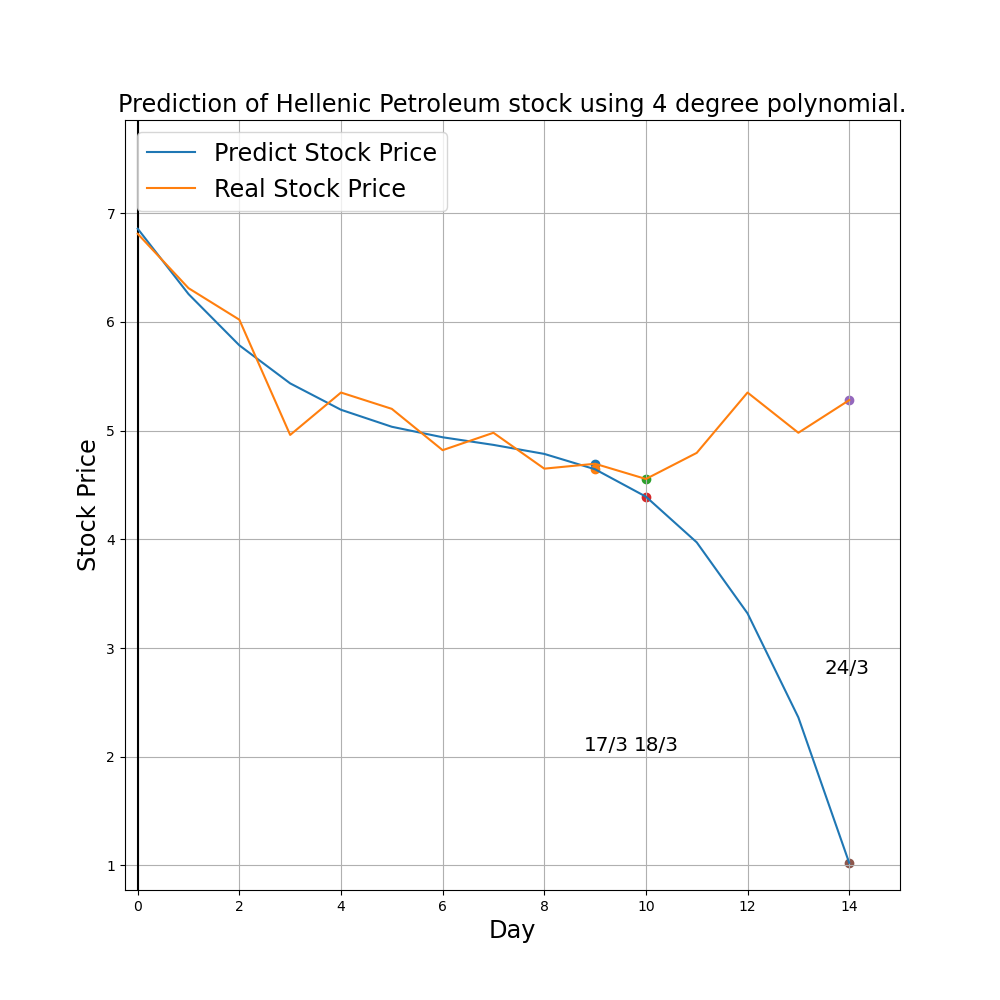
\includegraphics[scale=0.25]{hellenic_petroleum_stock_4_degree.png}    
        \caption{Διάγραμμα της πρόβλεψης καθώς και της πραγματικής τιμής κλεισίματος της μετόχης της εταιρείας 
        \textbf{ΕΛΛΗΝΙΚΑ ΠΕΤΡΕΛΑΙΑ} για το μοντέλο με βαθμό 4 για την περίοδο 4 με 24 Μαρτίου 2020.}
    \end{center}
\end{figure}

%2nd degree
%x_train = [0, 1, 2, 3, 4, 5, 6, 7, 8, 9]
%y_train = [6.81, 6.31, 6.02, 4.96, 5.35, 5.2, 4.82, 4.98, 4.65, 4.695]
%c = [6.755181818181812, -0.5074621212121171, 0.03185606060606017]
%x_test = [10, 11, 12, 13, 14]
%y_test = [4.555, 4.795, 5.35, 4.98, 5.28]
%y_predict = [4.87, 5.03, 5.25, 5.54, 5.89]
%rmse = 0.41320119494294816
%next meeting stock predict = 4.866166666666659
%real next meeting stock value = 4.555
%after 5 meetings stock predict = 5.894499999999967
%after 5 meetings real stock value =5.28
Πιο συγκεκριμένα, το πολυώνυμο 2ου βαθμού για την πρόβλεψη της τιμής κλεισίματος στις \textbf{18 Μαρτίου 2020} 
επιστρέφει την τιμή $4.866166666666659$ ενώ η πραγματική τιμή κλεισίματος για εκείνη την ημέρα ήταν
$4.555$. Για την πρόβλεψη 5 ημέρες μετά, δηλαδή στις \textbf{24 Μαρτίου 2020}, το μοντέλο επιστρέφει την τιμή 
$5.894499999999967$ ενώ η πραγματική τιμή κλεισίματος ήταν $5.28$. Για το \textlatin{\textbf{test set}} το
πολυώνυμο 2ου βαθμού πέτυχε \textbf{\textlatin{rmse} = 0.41320119494294816}, ενώ και για τις δύο προβλέψεις 
παρατηρούμε σχετικά καλές εκτιμήσεις με την δεύτερη να έχει μεγαλύτερη απόκλιση από την πρώτη. 

% 3rd degree
%x_train = [0, 1, 2, 3, 4, 5, 6, 7, 8, 9]
%y_train = [6.81, 6.31, 6.02, 4.96, 5.35, 5.2, 4.82, 4.98, 4.65, 4.695]
%c = [6.868013986013923, -0.7138733488732444, 0.09230186480183533, -0.004477466977464845]
%x_test = [10, 11, 12, 13, 14]
%y_test = [4.555, 4.795, 5.35, 4.98, 5.28]
%y_predict = [4.48, 4.22, 3.86, 3.35, 2.68]
%rmse = 1.5483780363486506
%next meeting stock predict = 4.482000000000168
%real next meeting stock value = 4.555
%after 5 meetings stock predict = 2.6787832167846926
%after 5 meetings real stock value =5.28
Πιο συγκεκριμένα, το πολυώνυμο 3ου βαθμού για την πρόβλεψη της τιμής κλεισίματος στις \textbf{18 Μαρτίου 2020} 
επιστρέφει την τιμή $4.482000000000168$ ενώ η πραγματική τιμή κλεισίματος για εκείνη την ημέρα ήταν
$4.555$. Για την πρόβλεψη 5 ημέρες μετά, δηλαδή στις \textbf{24 Μαρτίου 2020}, το μοντέλο επιστρέφει την τιμή 
$2.6787832167846926$ ενώ η πραγματική τιμή κλεισίματος ήταν $5.28$. Για το \textlatin{\textbf{test set}} το
πολυώνυμο 3ου βαθμού πέτυχε \textbf{\textlatin{rmse} = 1.5483780363486506}, ενώ παρατηρούμε για την πρώτη 
πρόβλεψη ότι είναι καλύτερη σε σχέση με την πρόβλεψη του πολυωνύμου 2ου βαθμού αλλά με την πρόβλεψη στις 24
Μαρτίου να έχει αρκετά μεγαλύτερη απόκλιση από την πραγματική τιμή κλεισίματος. 

% 4th degree
%x_train = [0, 1, 2, 3, 4, 5, 6, 7, 8, 9]
%y_train = [6.81, 6.31, 6.02, 4.96, 5.35, 5.2, 4.82, 4.98, 4.65, 4.695]
%c = [6.85674825174814, -0.666932789432366, 0.0659629953377673, 0.00021658896662852463, -0.00026078088578304094]
%x_test = [10, 11, 12, 13, 14]
%y_test = [4.555, 4.795, 5.35, 4.98, 5.28]
%y_predict = [4.39, 3.97, 3.32, 2.36, 1.02]
%rmse = 2.4409310013590737
%next meeting stock predict = 4.392499999999325
%real next meeting stock value = 4.555
%after 5 meetings stock predict = 1.0245979020847766
%after 5 meetings real stock value =5.28
Τέλος, το πολυώνυμο 4ου βαθμού για την πρόβλεψη της τιμής κλεισιματος στις \textbf{18 Μαρτίου 2020} 
επιστρέφει την τιμή $4.392499999999325$ ενώ η πραγματική τιμή κλεισίματος για εκείνη την ημέρα ήταν
$4.555$. Για την πρόβλεψη 5 ημέρες μετά, δηλαδή στις \textbf{24 Μαρτίου 2020}, το μοντέλο επιστρέφει την τιμή 
$1.0245979020847766$ ενώ η πραγματική τιμή κλεισίματος ήταν $5.28$. Για το \textlatin{\textbf{test set}} το
πολυώνυμο 4ου βαθμού πέτυχε \textbf{\textlatin{rmse} = 2.4409310013590737}, ενώ για τις προβλέψεις παρατηρούμε 
ότι η πρώτη εκτίμηση είναι σχετικά κοντά στην πραγματική τιμή, με την δεύτερη όμως να αποκλίνει με μεγαλύτερο 
σφάλμα απ' ότι στο πολυώνυμο 3ου βαθμού.

Συμπερασματικά, τα 3 μοντέλα καταντάσσονται με βάση το \textlatin{\textbf{RMSE}} στον παρακάτω πίνακα
\begin{center}
    \begin{tabular}{ |c|c|c| } 
     \hline
     Βαθμός Πολυωνύμου & \textlatin{RMSE} \\
     \hline
     2 & 0.41320119494294816 \\
     \hline
     3 & 1.5483780363486506 \\ 
     \hline
     4 & 2.4409310013590737 \\
     \hline
    \end{tabular}
\end{center}

ενώ σχετικά με τα διαγράμματα των \textit{σχήματων 8 και 9} παρατηρούμε ότι όσο ανεβαίνει ο βαθμός του 
πολυωνύμου έχουμε σχετικά καλύτερη προσέγγιση στο κέντρο του διαστήματος των σημείων εκπαίδευσης αλλά μεγαλύτερο 
σφάλμα όσο προχωράμε προς τα άκρα αυτού του διαστήματος, στο οποίο ανήκουν και οι ημερομηνίες για τις οποίες 
γίνεται η πρόβλεψη της τιμής κλεισίματος με αποτελέσμα να υπάρχει μεγαλύτερο σφάλμα σε σχέση με το πολυώνυμο 
2ου βάθμου και πάλι λόγω της κυρτότητας των πολυωνύμων 3ου και 4ου βαθμού. 
\end{document}